% Chapter Template

\chapter{Classical numerical results} % Main chapter title

\label{Chapter3} % Change X to a consecutive number; for referencing this chapter elsewhere, use \ref{ChapterX}


%----------------------------------------------------------------------------------------
%	SECTION 1
%----------------------------------------------------------------------------------------

In this section will we revisit the two classical results in computational finance the Binomial model and the Least Square Monte Carlo (LSM) approach. The models will both serve as reference for the Machine Learning model and provides insight into valuation of American options.


\section{Binomial Pricing model}
The Binomial model provides an intuitive and easy implementable model for valuing American and European options. The Binomial model comes handy, when no analytical model exists for american options. The Binomial model also has its limitations, because it is not suited for valuing path dependent options or options with several underlying factors. The key difference on the Binomial model and the other numerical procudures is that the Binomial model is build on a discrete framework. \\

The central concepts arbitrage and completeness from continuous time also work in the discrete time setup. The paper \parencite{binomial-Paper} which introduced the binomial model to option pricing came after the Black-Scholes model described in section \ref{Chapter2} \parencite{B-S-Paper}. The main reason for developing a model in discrete time, is that the the discrete time approach gives a simplified model in terms of the mathematics and highlights the essential concepts in option pricing theory. You can argue that the simpler mathematics in this model makes the binomial model more instructive and clear. Besides being easier to understand for non-mathematician it works nicely with other options than the European options like American options.\\

Eventhough we assume the stock price moves at discrete time instead in continuous time. It can actually be shown for a European Option that if the number of timesteps in the tree aproaches infinity, then the binomial model will converge to the continuous time closed form solution for a European option \parencite{binomial-Paper} \parencite{Hull}. Hence the binomial pricing model will be equivalent with the continuos time analytical pricing model derived by Fischer Black and Myron Scholes in the limit for european options \parencite{binomial-Paper}.\\

To value a american put option, we lay out all the possible path of the stock, based on the $S_0,\sigma$ and $T$. We need to specify the number of timesteps ($\Delta t = \frac{T}{N} \ where \ N=No. \ of  \ steps$) for the tree, where for each step, we add another possible value for the stock. We only add 1 more possibility for each timestep because the tree recombines. The precision for the algorithme increases with the number of steps and the option value stabilizes (see Figure \ref{fig:binConv}). For valuing an american put option, we value the exercise value at maturity (time T) for all possible outcomes for the stock. Then we work backward in the tree by comparing intrinsic value with the conditional expectation, where we choose the maximum of these two \parencite{Hull}. 
 
\begin{figure}[th]
\centering
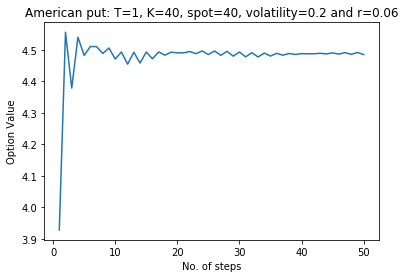
\includegraphics{Figures/binConv.png}
\decoRule
\caption[Convergence of Binomial model]{}
\label{fig:binConv}
\end{figure}



%-----------------------------------
%	SUBSECTION 1
%-----------------------------------
\subsection{Mathematics in Binomial Pricing model}
The mathematics behind the binomial model are simpel and we will this section to provide the basic. For each time step ($\Delta t$), we assume the stock (S) can move up (u) or down (d). In order to avoid arbitrage we find the risk neutral measure q for the binomial tree. The risk neutral measure q is chosen s.t. the expected return is the risk-free rate r.

\begin{theorem}\label{RNVF-Discrete}
\textbf{Risk-neutral valuation formula in discrete time. }
Assume there exists a risk free asset. Then the market is arbitage free if and only if there exists a risk neutral measure $Q \sim P$ s.t.
\begin{align}
s= \exp(- r \Delta t) \cdot E^Q[S(t+\Delta t)|S(t)=s] 
\end{align}
Where $\Delta t$ is a single timestep.
\end{theorem}
From the above theorem, we can calculate the risk neutral mesure as:\\
$$q=\frac{e^{\Delta t}-d}{u-d}$$

The d and u is chosen s.t. they match volatility. So we choose:
$$u= \exp(\sigma \sqrt{\Delta t}) \quad d= \exp(-\sigma \sqrt{\Delta t})$$
Now we have determined the three parameters needed for constructing a binomial tree \parencite{binomial-Paper} \parencite{Hull} \parencite{finKont}.\\

We want to value an American put option, hence we need to work backward in the tree and comparing in each node the intrinsic value with the conditional expection (see theorem \ref{RNVF-Discrete}) by:
\begin{equation}
max\{ K-S(t), e^{-r \Delta t} \exp(- r \Delta t) \cdot E^Q[P(t+\Delta t,T)|P(t,T)=p] \}
\end{equation}
The comparision will be applied for every node in each timestep $\Delta t$  and all the way back in time to the initialization date. By this precedure we get present value of the American option at initialization.

%-----------------------------------
%	SUBSECTION 2
%-----------------------------------


%----------------------------------------------------------------------------------------
%	SECTION 2
%----------------------------------------------------------------------------------------

\section{Least Square Monte Carlo Method}
The other classical result in this section is somewhat more technical without familarity with statistics, but on the other hand the least square method and linear regression is a well known and testet in statistics. In our setting we regress the expected payoff by continuation of the contract and compare it to the intrinsic value. The dependent variable is the expected value and the independent variables is a set of othogonal basis functions in $L^2(\Omega, \mathcal{F}, Q)$. Typical choices for basis functions could be weighted Laguerre -, Hermit -, and Jacob polynomials. This kind of regression is a nonlinear expansion of the linear model. In order to create data, we will simulate paths according to the underlying risky asset. 

\subsection{Application of the LSM method}
We want to valuate an American put option with a stock as underlying asset. We assume the stock follows a GBM: $dS(t)=rSdt + \sigma S dW_t$ where $\sigma$ and r is constant (see solution to SDE equation \ref{GBM}). We simulate 100.000 paths for the stock, where 50.000 of the paths is antithetic of the first 50.000 using 50 exercise points per year.

\parencite{lsm}  

\section{Comparision}

